%!TEX root = main.tex
\tvcg{\section{Methods} \label{methods}}
%\subsection{Evaluation Methods For Visualization Systems}
\tvcg{In this section, we will first provide a brief overview of existing evaluation methodology for visualization system, then describe our chosen research methodology in this paper.}
\tvcg{\subsection{Methodology Background\label{methodology_relatedwork}}}
\par Visualization systems are often evaluated using controlled studies that measure the user's performance against an existing visualization baseline~\cite{Plaisant2004}. Cognitive measures such as insight time~\cite{North2006,Yi2008} have been developed to capture how well users perform on a task against existing baselines. However, since the operations, hypotheses generated, and insights obtained through exploratory analysis are variable and subjective to individual users and their analytic goals, it is impossible to define tasks beforehand and compare across control groups. Techniques such as artificially inserting ``insights'' or setting predefined tasks for example datasets work well for objective tasks, such as debugging data errors~\cite{kandel2011wrangler,Patel2010}, but this contrived method is unsuitable for trying to learn about the types of real-world queries a user may want to pose on a VQS. \techreport{In order to make the user study more realistic, we opted for a qualitative evaluation where we allowed participants to bring a dataset that they have a vested interest in to address an unanswered research question.}
\par Due to the unrealistic nature of controlled studies, many have proposed using a more multi-faceted, ethnographic approach to understand how analysts perform visual data analysis and reasoning~\cite{Plaisant2004,lam2012empirical,shneiderman2006strategies,munzner2009nested,Sedlmair2012}. For example, multi-dimensional, in-depth, long-term case studies (MILCs) advocate the use of interviews, surveys, logging and other empirical artifacts to create a holistic understanding of how a visualization system is used in its intended environment \cite{shneiderman2006strategies}. Some papers have explored designing visualization and collaborative tools for scientific workflows through individual case studies, e.g.,~\cite{Poon2008,Chen2016}. Similarly, in our work, real-world case studies help us situate how VQSs could be used in the context of an existing analysis workflow.  
\par We adopt {\em participatory design} practices in this work: participatory design ``allows potential users to 
 participate in the design of a system that they will ultimately use''~\cite{Gould1983,Muller1993}. Participatory design has been successfully used in the development of interactive visualization systems in the past~\cite{Aragon2008,Chuang2012}. \tvcg{Sedlmair et al. \cite{Sedlmair2012} highlights the benefits and pitfalls of design study. They advocate that design study methodology is suitable for use cases in which the data is available for prototyping, but the task is only partially known and information is partially in the user's head. In that regard, our scientific use cases with VQS is well-suited for a design study methodology, as we learn about the scientist's data and analysis requirements and design interactions that helps users translate their ``in-the-head'' specifications into actionable visual queries.} %\cut{In this work, we collaborated with scientists early on to develop features in \zv that address their analysis needs.}  
\tvcg{\subsection{Our Approach}}
\par We adopted a mixed methods research methodology that draws inspiration from ethnographic methods, iterative and participatory design, and controlled studies~\cite{jorgensen_2008,miller_salkind_miller_2002,shneiderman2006strategies,Muller1993} to understand how VQSs can accelerate scientific data analysis. \tvcg{Our methodology was designed to address the research questions outlined in the introduction.} Working with researchers from three different scientific research groups, we identified the needs and challenges of scientific data analysis and the potential opportunities for VQSs to fit in, via interviews and cognitive walkthroughs {\em (RQ1)}. We further extended an existing VQS, \zv, with features for scientists via participatory design {\em (RQ2)}  
\par \tvcg{Given our early conversations with the participants, we built a basic VQS to serve as the functional prototype in the design study. As shown in Figure \ref{oldZV}, this early version of \zv allowed users to sketch a pattern or drag-and-drop an existing visualization as a query, then the system would return visualizations that had the closest Euclidean distance from the queried pattern. \zv also displayed representative and outlier patterns to help provide an overview of typical trends.
	\begin{figure}[ht!]
	\centering
	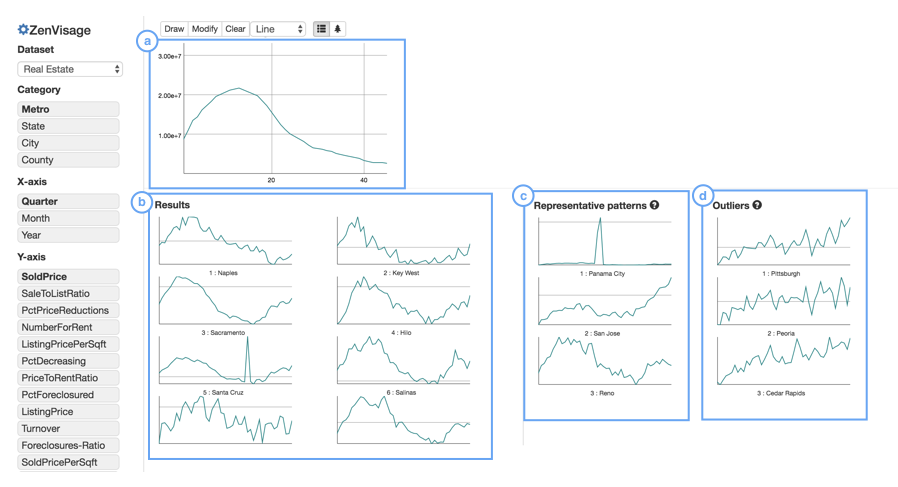
\includegraphics[width=\linewidth]{figures/oldZV_nozql.png}
	\caption{The \zv prototype allowed users to sketch a pattern in (a), which would then return (b) results that had the closest Euclidean distance from the sketched pattern. The system also displays (c) representative patterns obtained through K-means clustering and (d) outlier patterns to help the users gain an overview of the dataset. \tvcg{\zv also has a sophisticated query language, ZQL, that we did not employ for this study. The details of the system is described in our previous work \cite{Siddiqui2017,Siddiqui2017VLDB}, which focused on the systems and scalability aspects of the VQSs.}}
	\label{oldZV}
	\end{figure}
\par The use of functional prototypes is common in participatory design to provide a starting point for the participants.} For example, Ciolfi et al.\cite{Ciolfi2016} studied two different alternatives to co-design (starting with open brief versus functional prototype) in the development of museum guidance systems and found that while both approaches were equally fruitful, functional prototypes can make addressing a specific challenge more immediate and focused (in our case the challenge is making comparison across large numbers of visualizations as we found in through informal discussions with practitioners). Our motivation for providing a functional prototype at the beginning of the participatory design sessions is to showcase capabilities of VQSs. Especially since VQSs are not uncommon in the existing workflow of these scientists, participants may not be able to imagine their use cases without a starting point. %\sout{our prototypical VQS, since it is open-source, has both canvas-based querying capabilities as well as visualization recommendations. (\zv also has a sophisticated query language, ZQL, that we did not employ.)} 
\par After incorporating desired features into \zv over the period of a year, we conducted a qualitative evaluation to study how our improved VQS affected the way the users explore their data{\em (RQ3,4)}. \cut{It is interesting to note that not all of the features suggested by the participants were found to be useful during our evaluation.}